\section{Identification study: design}\label{sec:design}

\subsection{Question}

Given a different photo of the same person, with part of the face covered, does a model still identify that person among \N{n_test_identities} people it never trained on? How fast does identification fall with the occluder's size, place, and fill? And do the project's attention layer and occlusion augmentation help a small network when every model sees the same aligned face crop? The study's settings are in its configuration file, which the run log records; there is no validation split; and three primary contrasts are defined in the study code (Section~\ref{sec:metrics}).

\subsection{Data, labels, and split}

The images are the \N{n_label_images} CelebA-HQ pictures~\cite{karras2018pggan,liu2015celeba} at 256$\times$256 (a Kaggle copy~\cite{kagglecelebahq}). Identity labels come from CelebA-Dialog~\cite{jiang2021talk,lee2020maskgan}: \N{n_identities} identities. The Kaggle copy numbers its files in an order unrelated to the CelebA-HQ index that the labels use, so each file was matched to CelebA-Dialog's own copy of the images by thumbnail correlation: all \N{n_label_images} matched, with a lowest match correlation of \N{map_min}, and \N{map_second} images took a candidate other than their best to keep the map one-to-one. On \N{fit_n} aligned crops, each matched against the others, ArcFace's rank-1 among the crops with a same-label partner in the sample is \N{fit_file_r1} when the labels are read by file number and \N{fit_map_r1} through the map. Before any training, the run checked that both pretrained models reach a clean-probe rank-1 of at least \N{label_floor}; they reached \N{lc_sf} (SFace) and \N{lc_arc} (ArcFace).

Identities with at least two images are eligible. With seed \N{seed}, \N{n_test_identities} test identities were drawn; each keeps its lowest-numbered image as its gallery image, and its other images are probes. Every other identity with at least two images is used for training, so no identity is in both. Before alignment, that gives \N{role_train} training images, \N{n_gallery} gallery images, and \N{role_probe} probes, with \N{role_unused} images of single-image identities unused. Alignment failed on \N{n_not_aligned} images (\N{drop_train} training images and \N{drop_probe} test image), leaving \N{n_train_images} training images of \N{n_train_identities} identities (\N{train_per_id} per identity on average) and \N{n_probes} probes of all \N{n_test_identities} test identities (\N{probes_per_id} per identity). Rank-1 chance is \N{chance}\%.

\subsection{Alignment and occluders}

YuNet~\cite{wu2023yunet} (score threshold \N{yunet_thr}) finds the face and five landmarks on the clean 256$\times$256 image, and OpenCV's \texttt{alignCrop} maps them onto the standard \N{crop}$\times$\N{crop} ArcFace template. Occluders are drawn on this crop afterward, so they never change where the face is found: recognition here has oracle alignment, likely an upper bound for a real pipeline, whose detector (a Haar cascade, in the re-creation of Section~\ref{sec:original}) fails first.

There are \N{n_conditions} identity conditions (Fig.~\ref{fig:occluders}): centered black squares covering 0, 5, 10, 15, 20, 25, 30, 40, 50, and 60\% of the crop (the side is the integer part of the square root of the area, so 20\% is a \N{side_s20}-pixel square); an eye band (rows \N{eye_r0} to \N{eye_r1}\% of the crop, \N{eye_area}\% of its area); a lower band (rows \N{low_r0} to \N{low_r1}\%, \N{low_area}\%); a 20\% black square at a seeded random position per image (``off-center''); and centered squares filled with gray (value 128) or uniform noise at 20 and 40\%. The same-image control occludes each gallery image with a centered square at 0, 5, 10, 20, 30, or 50\% of the crop and matches it back against the gallery. All occluders are synthetic.

\begin{figure}[t]
\centering
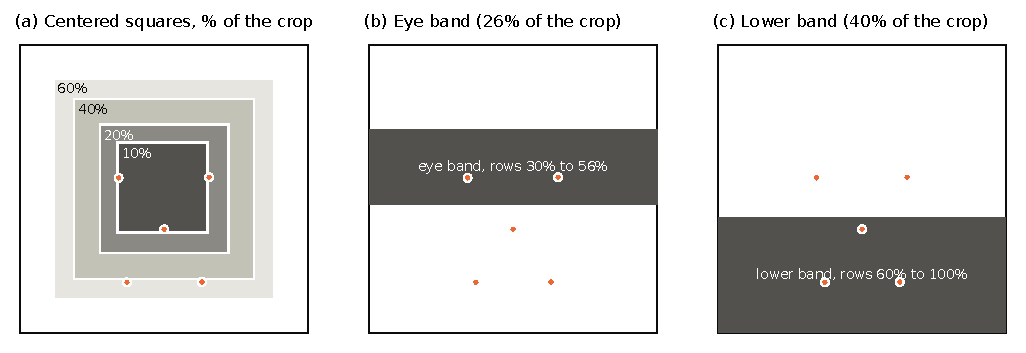
\includegraphics[width=\columnwidth]{figures/fig_occluders.pdf}
\caption{The study's occluders on the \N{crop}$\times$\N{crop} aligned crop, drawn on an empty frame with the five landmark positions of the alignment template (dots: eyes, nose tip, mouth corners); no face image is shown. (a) Centered black squares at 10, 20, 40, and 60\% of the crop (5 to 50\% are drawn the same way). (b) Eye band. (c) Lower band. Not drawn: the off-center 20\% square, at a random position per image, and the gray and noise fills, which use the centered 20\% and 40\% squares. The 20\% square covers both eye landmarks and the nose tip; the lower band covers the nose tip and the mouth corners.}
\label{fig:occluders}
\end{figure}

\subsection{Models}

Table~\ref{tab:arms} lists the arms. The pretrained models are SFace~\cite{zhong2021sface} (the OpenCV Zoo file DeepFace uses) and InsightFace's ArcFace ResNet-50 trained on WebFace600K (\texttt{w600k\_r50} from the \texttt{buffalo\_l} pack~\cite{insightface}), both run through OpenCV's DNN module on the CPU and matched by cosine similarity. Raw pixels are matched by Euclidean distance, on the crop or on the frame downsampled to \N{frame_small}$\times$\N{frame_small}. The original model is the saved network of Section~\ref{sec:original}, on its own input: whole 256$\times$256 frames scaled to $[0,1]$, unnormalized embeddings, and Euclidean distance. The frame-based arms use the original's 21 frame-square levels instead of crop conditions.

The trained arms are the project's network (Section~\ref{sec:original}) with the attention layer on or off, crossed with occlusion augmentation on or off. They are trained on the training identities' crops, scaled to $[-1,1]$, with the CosFace loss (scale \N{cos_s}, margin \N{cos_m})~\cite{wang2018cosface}. Augmentation draws the project's centered black square, with coverage uniform from \N{occ_lo} to \N{occ_hi}\%, on each training image with probability \N{occ_prob}\%; the eye band, lower band, off-center square, and gray and noise fills never appear in training. A fifth arm uses a batch-hard triplet loss~\cite{hermans2017defense} on L2-normalized embeddings (margin \N{tri_m}, \N{tri_p} identities of \N{tri_k} images per batch) with attention and augmentation on; it is not the original's recipe of random negatives and margin \N{orig_margin}. All runs use horizontal flips, AdamW~\cite{loshchilov2019decoupled} with learning rate \N{lr} and weight decay \N{wd}, one warmup epoch and then a cosine schedule~\cite{loshchilov2017sgdr}, \N{epochs} epochs, batch size \N{batch}, and bfloat16 autocast, with \N{n_seeds} seeds each: \N{n_runs} runs on one NVIDIA A10 GPU.

\begin{table}[t]
\caption{Arms of the study. Crop = the \N{crop}$\times$\N{crop} aligned crop; frame = the whole image. ``Both'' = attention and occlusion augmentation. Each trained CNN has \N{n_seeds} seeds.}
\label{tab:arms}
\centering\small
\setlength{\tabcolsep}{3pt}
% Generated by make_numbers.py. Do not edit.
\begin{tabular}{@{}llll@{}}
\toprule
Model & Training & Input & Match \\
\midrule
ArcFace R50 & pretrained & crop & cosine \\
SFace & pretrained & crop & cosine \\
Crop pixels & none & crop & $L_2$ \\
Frame pixels & none & frame, 128 px & $L_2$ \\
Original model & saved & frame, 256 px & $L_2$ \\
CNN, neither & CosFace & crop & cosine \\
CNN, attention & CosFace, att. & crop & cosine \\
CNN, augmentation & CosFace, aug. & crop & cosine \\
CNN, both & CosFace, att., aug. & crop & cosine \\
CNN, both, triplet & triplet, att., aug. & crop & cosine \\
\bottomrule
\end{tabular}

\end{table}

\subsection{Metrics, intervals, and tests}\label{sec:metrics}

Rank-1 is the share of probes whose own identity's gallery image scores highest among the \N{n_gallery}. Verification uses every probe--gallery pair. Its main reading fixes a threshold once per model (per seed for the trained CNNs), on clean identity probes, at a false accept rate (FAR) of \N{far1}\% or \N{far01}\%, and applies it to every condition, as a deployed system would; the true accept rate (TAR) and the actual FAR under each condition are reported at that threshold. A second reading, labeled ``re-set'', sets the threshold separately on each condition's own impostor scores. The same-image control gives the gap between the original protocol and identification for each model.

Intervals are 95\% percentile bootstrap intervals~\cite{efron1993bootstrap} from \N{resamples} resamples. Each resample draws test identities with replacement and, for each trained configuration, its \N{n_seeds} seeds with replacement, so the intervals carry training-seed variation as well as identity sampling; with \N{n_seeds} seeds, that part is coarse. Contrasts are paired by test identity within each resample, while each configuration's seeds are drawn separately, as if its runs were independent of the others'.

Three primary contrasts on identity rank-1 are defined in the study code (\texttt{study/analyze.py}), each a main effect (the mean of the factor's effect with and without the other factor):
\begin{itemize}
\item P1: augmentation, over the \N{n_trained_squares} centered black squares from 10 to 50\% (the occluder it trains with);
\item P2: augmentation, over the \N{n_unseen} occluders never seen in training (both bands, the off-center square, and the four fills);
\item P3: attention, over all \N{n_p3} occluded conditions of P1 and P2.
\end{itemize}
Each is claimed only if its Holm-adjusted~\cite{holm1979simple} bootstrap $p$-value is below 0.05. The $p$-values are two-sided with the add-one correction~\cite{davison1997bootstrap}, $2(1+k)/(B+1)$, where $k$ counts resamples on the far side of zero and $B=\N{resamples}$. When no resample crosses zero, the value sits at its floor, $2/\N{resamples1}\approx\N{p_floor}$, the smallest value \N{resamples} resamples can give, and it is quoted as $p<\N{P1_p}$ (Holm $p<\N{P1_holm}$). The primary contrasts are also tested with seeds as the unit (Section~\ref{sec:ablation}). Each primary contrast is also given as the range over all \N{combos} ways to take one seed per configuration. Everything else, including the main effect at each single condition and the simple contrasts behind them, is descriptive and unadjusted.
